\begin{figure}
  \centering
  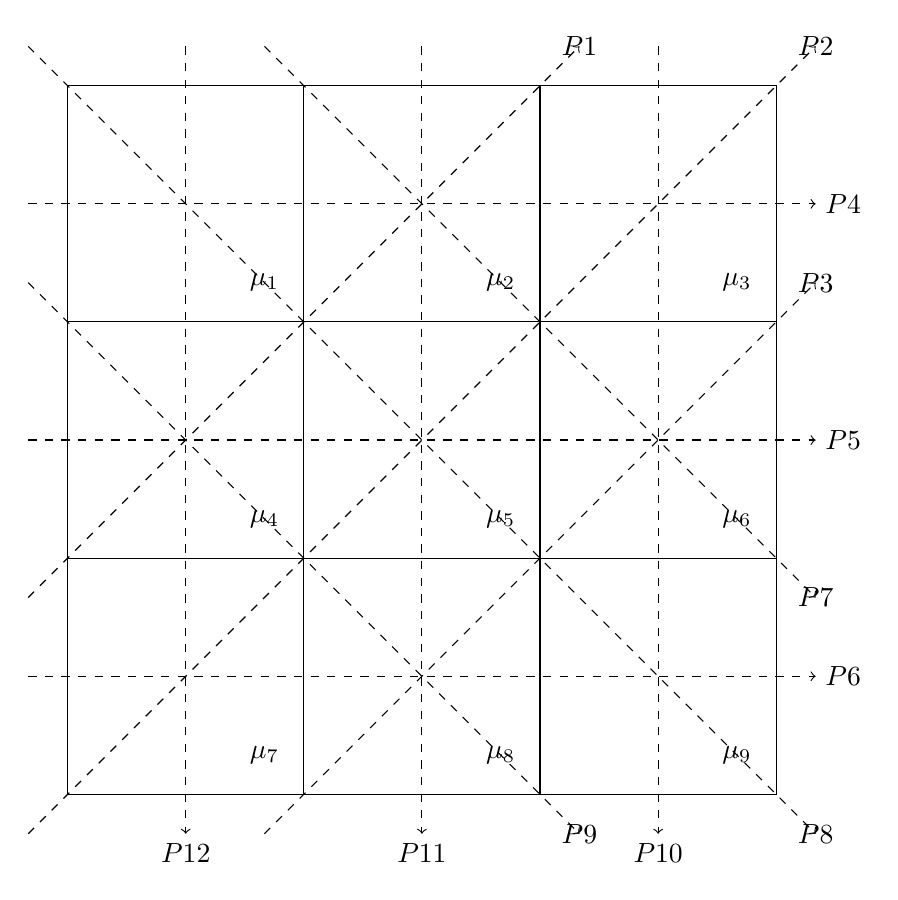
\begin{tikzpicture}
    \draw (0,9) -- (3,9) -- (3,6) -- (0,6) -- (0,9); % wuerfel 1
    \draw (3,9) -- (6,9) -- (6,6) -- (3,6) -- (3,9); % wuerfel 2
    \draw (6,9) -- (9,9) -- (9,6) -- (6,6) -- (6,9); % wuerfel 3
    \draw (0,6) -- (3,6) -- (3,3) -- (0,3) -- (0,6); % wuerfel 4
    \draw (3,6) -- (6,6) -- (6,3) -- (3,3) -- (3,6); % wuerfel 5
    \draw (6,6) -- (9,6) -- (9,3) -- (6,3) -- (6,6); % wuerfel 6
    \draw (0,3) -- (3,3) -- (3,0) -- (0,0) -- (0,3); % wuerfel 7
    \draw (3,3) -- (6,3) -- (6,0) -- (3,0) -- (3,3); % wuerfel 8
    \draw (6,3) -- (9,3) -- (9,0) -- (6,0) -- (6,3); % wuerfel 9
    \draw (2.5,6.5) node {$\symbf{\mu}_{1}$};
    \draw (5.5,6.5) node {$\symbf{\mu}_{2}$};
    \draw (8.5,6.5) node {$\symbf{\mu}_{3}$};
    \draw (2.5,3.5) node {$\symbf{\mu}_{4}$};
    \draw (5.5,3.5) node {$\symbf{\mu}_{5}$};
    \draw (8.5,3.5) node {$\symbf{\mu}_{6}$};
    \draw (2.5,0.5) node {$\symbf{\mu}_{7}$};
    \draw (5.5,0.5) node {$\symbf{\mu}_{8}$};
    \draw (8.5,0.5) node {$\symbf{\mu}_{9}$};
    % projektionsrichtungen
    \draw[->, dashed] (-0.5, 2.5) -- (6.5, 9.5) node {$P1$};
    \draw[->, dashed] (-0.5,-0.5) -- (9.5, 9.5) node {$P2$};
    \draw[->, dashed] (2.5, -0.5) -- (9.5, 6.5) node {$P3$};
    \draw[->, dashed] (-0.5, 7.5) -- (9.5, 7.5) node[right] {$P4$};
    \draw[->, dashed] (-0.5, 4.5) -- (9.5, 4.5) node[right] {$P5$};
    \draw[->, dashed] (-0.5, 1.5) -- (9.5, 1.5) node[right] {$P6$};
    \draw[->, dashed] ( 2.5, 9.5) -- (9.5, 2.5) node {$P7$};
    \draw[->, dashed] (-0.5, 9.5) -- (9.5,-0.5) node {$P8$};
    \draw[->, dashed] (-0.5, 6.5) -- (6.5,-0.5) node {$P9$};
    \draw[->, dashed] ( 1.5, 9.5) -- (1.5,-0.5) node[below] {$P12$};
    \draw[->, dashed] ( 4.5, 9.5) -- (4.5,-0.5) node[below] {$P11$};
    \draw[->, dashed] ( 7.5, 9.5) -- (7.5,-0.5) node[below] {$P10$};
  \end{tikzpicture}
  \caption{Abbildung der zwölf Projektionsrichtungen in einer Würfelebene mit je 9 kleineren Würfeln.}
  \label{fig:projection}
\end{figure}
